\section{System Overview}

\begin{frame}{LG-Loc System Architecture}
    \begin{columns}
        \begin{column}{.6\textwidth}
            \begin{itemize}
                \item Users launch the localization application upon entering a building and obtains his location;
                \item Application requests the building's landmark graph stored in the server;
                \item Data are preprocessed through a low-pass filter;
                \item Data used for landmark detection and location estimation;
                \item Initial location obtained via:
                    \begin{itemize}
                        \item WiFi fingerprinting (if database is available);
                        \item HMM-based algorithm (if database is unavailable).
                    \end{itemize}
            \end{itemize}
        \end{column}
        \begin{column}{.4\textwidth}
            \begin{figure}[t]
                \centering
                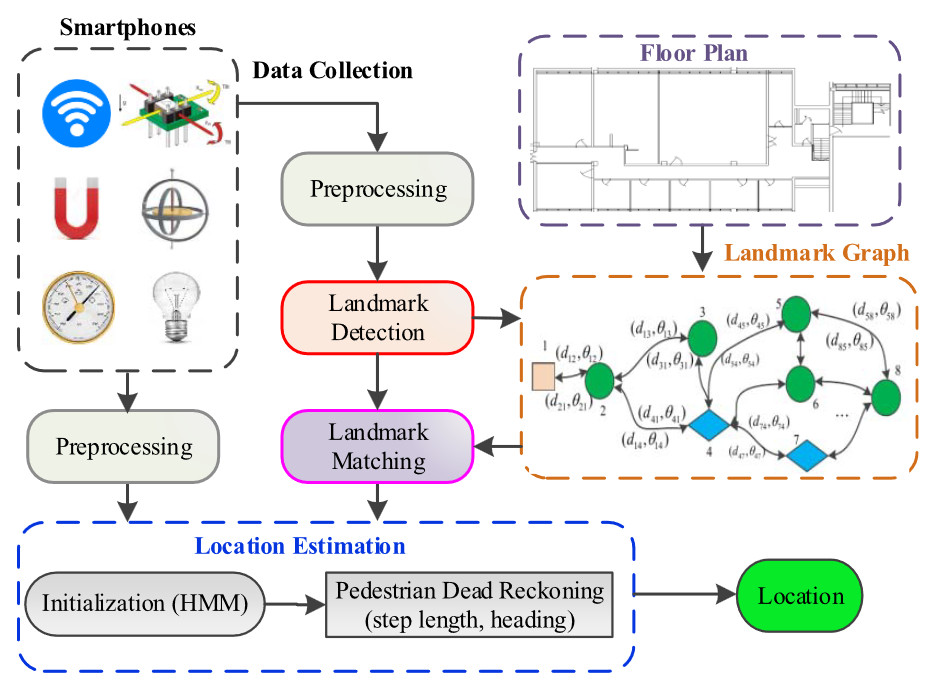
\includegraphics[width=\linewidth]{images/sys.jpg}
                \caption{System architecture of LG-Loc}
                \label{fig:sys}
            \end{figure}
        \end{column}
    \end{columns}
\end{frame}